Serieregulatorer har en eller flere enheter plassert i serie med lasten.

\begin{figure}[H]
  \centering
  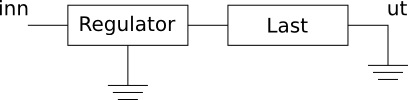
\includegraphics[width=0.67\textwidth]{./img/serie-boks}
  \caption{Regulatoren er i serie med lasten}
\end{figure}

En implementasjon av en serieregulator er en pass transistor regulator.

\begin{circuitikz} \draw
(4,3) node[npn,rotate=90] (npn) {}
(npn.base)

(0,3) node[label=$V_{inn}$] {}
      to[short, o-] (3.3,3)
(2,3) -- (2,2)
      to[R] (4,2)
      -- (4,2.2)

(4,0) node[ground] {}
      to[zD*] (4,2)

(4.7,3) node[label=$V_{ut}$] {}
      to[R, l=$R_L$, o-] (7,3)
      -- (7,2.5)
      node[ground] {}
      ;
\end{circuitikz}

Spenningsfall over $V_{BE}$ gjør at ledningsevnen til transistoren øker
og en relativt stabil spennings opprettholdes.

Merk! Denne kretsen har hverken feilbehandling eller sikring.
